\documentclass[journal,12pt,twocolumn]{IEEEtran}
 \usepackage{setspace}
 \usepackage{gensymb}
 \usepackage{graphicx}
 \singlespacing
\graphicspath{ {/user/adarshsrivastava/desktop/Matrix Theory/Assignemnt_5} }
 \usepackage[cmex10]{amsmath}
 \usepackage{amsthm}
 \usepackage{hyperref}
 \usepackage{mathrsfs}
 \usepackage{txfonts}
 \usepackage{stfloats}
 \usepackage{bm}
 \usepackage{cite}
 \usepackage{cases}
 \usepackage{subfig}
 \usepackage{longtable}
 \usepackage{multirow}
 \usepackage{enumitem}
 \usepackage{mathtools}
 \usepackage{steinmetz}
 \usepackage{tikz}
 \usepackage{circuitikz}
 \usepackage{verbatim}
 \usepackage{tfrupee}
 \usepackage[breaklinks=true]{hyperref}
 \usepackage{tkz-euclide}
 \usetikzlibrary{calc,math}
 \usepackage{listings}
     \usepackage{color}                                            %%
     \usepackage{array}                                            %%
     \usepackage{longtable}                                        %%
     \usepackage{calc}                                             %%
     \usepackage{multirow}                                         %%
     \usepackage{hhline}                                           %%
     \usepackage{ifthen}                                           %%
     \usepackage{lscape}     
 \usepackage{multicol}
 \usepackage{chngcntr}
 \DeclareMathOperator*{\Res}{Res}
 \renewcommand\thesection{\arabic{section}}
 \renewcommand\thesubsection{\thesection.\arabic{subsection}}
 \renewcommand\thesubsubsection{\thesubsection.\arabic{subsubsection}}
 \renewcommand\thesectiondis{\arabic{section}}
 \renewcommand\thesubsectiondis{\thesectiondis.\arabic{subsection}}
 \renewcommand\thesubsubsectiondis{\thesubsectiondis.\arabic{subsubsection}}
 \hyphenation{op-tical net-works semi-conduc-tor}
 \def\inputGnumericTable{}                                 %%
 \lstset{
 %language=C,
 frame=single, 
 breaklines=true,
 columns=fullflexible
 }
 \begin{document}
 \newtheorem{theorem}{Theorem}[section]
 \newtheorem{problem}{Problem}
 \newtheorem{proposition}{Proposition}[section]
 \newtheorem{lemma}{Lemma}[section]
 \newtheorem{corollary}[theorem]{Corollary}
 \newtheorem{example}{Example}[section]
 \newtheorem{definition}[problem]{Definition}
 \newcommand{\BEQA}{\begin{eqnarray}}
 \newcommand{\EEQA}{\end{eqnarray}}
 \newcommand{\define}{\stackrel{\triangle}{=}}
 \bibliographystyle{IEEEtran}
 \providecommand{\mbf}{\mathbf}
 \providecommand{\pr}[1]{\ensuremath{\Pr\left(#1\right)}}
 \providecommand{\qfunc}[1]{\ensuremath{Q\left(#1\right)}}
 \providecommand{\sbrak}[1]{\ensuremath{{}\left[#1\right]}}
 \providecommand{\lsbrak}[1]{\ensuremath{{}\left[#1\right.}}
 \providecommand{\rsbrak}[1]{\ensuremath{{}\left.#1\right]}}
 \providecommand{\brak}[1]{\ensuremath{\left(#1\right)}}
 \providecommand{\lbrak}[1]{\ensuremath{\left(#1\right.}}
 \providecommand{\rbrak}[1]{\ensuremath{\left.#1\right)}}
 \providecommand{\cbrak}[1]{\ensuremath{\left\{#1\right\}}}
 \providecommand{\lcbrak}[1]{\ensuremath{\left\{#1\right.}}
 \providecommand{\rcbrak}[1]{\ensuremath{\left.#1\right\}}}
 \theoremstyle{remark}
 \newtheorem{rem}{Remark}
 \newcommand{\sgn}{\mathop{\mathrm{sgn}}}
 \providecommand{\abs}[1]{\left\vert#1\right\vert}
 \providecommand{\res}[1]{\Res\displaylimits_{#1}} 
 \providecommand{\norm}[1]{\left\lVert#1\right\rVert}
 %\providecommand{\norm}[1]{\lVert#1\rVert}
 \providecommand{\mtx}[1]{\mathbf{#1}}
 \providecommand{\mean}[1]{E\left[ #1 \right]}
 \providecommand{\fourier}{\overset{\mathcal{F}}{ \rightleftharpoons}}
 %\providecommand{\hilbert}{\overset{\mathcal{H}}{ \rightleftharpoons}}
 \providecommand{\system}{\overset{\mathcal{H}}{ \longleftrightarrow}}
 	%\newcommand{\solution}[2]{\textbf{Solution:}{#1}}
 \newcommand{\solution}{\noindent \textbf{Solution: }}
 \newcommand{\cosec}{\,\text{cosec}\,}
 \providecommand{\dec}[2]{\ensuremath{\overset{#1}{\underset{#2}{\gtrless}}}}
 \newcommand{\myvec}[1]{\ensuremath{\begin{pmatrix}#1\end{pmatrix}}}
 \newcommand{\mydet}[1]{\ensuremath{\begin{vmatrix}#1\end{vmatrix}}}
 \numberwithin{equation}{subsection}
 \makeatletter
 \@addtoreset{figure}{problem}
 \makeatother
 \let\StandardTheFigure\thefigure
 \let\vec\mathbf
 \renewcommand{\thefigure}{\theproblem}
 \def\putbox#1#2#3{\makebox[0in][l]{\makebox[#1][l]{}\raisebox{\baselineskip}[0in][0in]{\raisebox{#2}[0in][0in]{#3}}}}
      \def\rightbox#1{\makebox[0in][r]{#1}}
      \def\centbox#1{\makebox[0in]{#1}}
      \def\topbox#1{\raisebox{-\baselineskip}[0in][0in]{#1}}
      \def\midbox#1{\raisebox{-0.5\baselineskip}[0in][0in]{#1}}
 \vspace{3cm}
 \title{Assignment 5}
 \author{Rubeena Aafreen}
 \maketitle
 \newpage
 \bigskip
 \renewcommand{\thefigure}{\theenumi}
 \renewcommand{\thetable}{\theenumi}
 The link to the solution is
 \begin{lstlisting}
  https://github.com/rubeenaafreen20/EE5609/tree/master/Assignment3
 \end{lstlisting}
 \begin{abstract}
 This documents solves a problem based on circles.
 \end{abstract}
  \section{Problem}
 Find the points on the curve $\vec{x}^{T}\vec{x}-2\myvec{1 & 0}\vec{x}-3=0$ at which the tangents are parallel to the x-axis
\section{Solution}
General equation of circle is 
\begin{align}
    \vec{x}^T\vec{x}+ 2\vec{u}^T\vec{x}+f = 0
    \label{eq:1}
\end{align}
The centre and the radius can be obtained as,
 \begin{align}
\vec{u}=\myvec{-1\\0}\\
f=-3\\
\vec{c}=-\vec{u}=\myvec{1\\0}\\
 r=\sqrt{\norm{\vec{u}}^2-f}=2
 \end{align}
$\because$ The tangents are parallel to the x-axis, their direction and normal vectors, $\vec{m}$ and $\vec{n}$ are respectively,
\begin{align}
\vec{m}=\myvec{1\\0}\\
\vec{n}=\myvec{0\\1}
\end{align}
For a circle, given the normal vector $\vec{n}$, the tangent points of contact to circle given by equation \eqref{eq:1}  are given by
\begin{align}
    \vec{q_i}=(\kappa_i \vec{n}-\vec{u}), i=1,2
    \label{eq:2}
\end{align}
where
\begin{align}
    \kappa_i=\pm \sqrt{\frac{\vec{u^T}\vec{u}-f}{\vec{n^T}\vec{n}}}\\
    \kappa=\pm \sqrt{\frac{\myvec{-1 & 0}\myvec{-1\\0}-(-3)}{\myvec{0 & 1} \myvec{0\\1}}}\\
 \implies \kappa=\pm \sqrt{\frac{4}{1}}\\
    \implies \kappa=\pm 2      
\end{align}
and from \eqref{eq:2} , the point of contact $\vec{q_i}$ are,
\begin{align}
    \vec{q_1}=2\myvec{0\\1}-\myvec{-1\\0}\\
    =\myvec{1\\2}\\
    \vec{q_2}=-2\myvec{0\\1}-\myvec{-1\\0}\\
    =\myvec{1\\-2}
\end{align}
 \begin{figure}[h!]
 \renewcommand \thefigure{1}
	\centering
	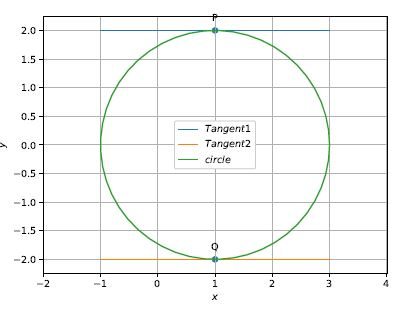
\includegraphics[width=\columnwidth]{fig1.JPG}
	\caption{Figure depicting tangents of circle parallel to x-axis}
	\label{fig1}
\end{figure}
 \end{document}